\chapter{Methodology}
\section{Project Scope \& Goal}
In terms of project scope it was necessary to aim for something ideally with quite a few moving parts, with use of as much new technology as possible. Initial ideas consisted of the likes of machine learning or the use of computer vision. Possible academic solutions were examined, with emphasis on security and encryption. One idea was a web store for a local farmers market, which with three people in the group, was declined as there would be a possible factor of work-load starvation between team members. 
\\ Based upon those initial concepts an idea was toyed with in terms of an agricultural application which would use a mixture of drone monitoring, computer vision and artificial intelligence to track the location and behaviour of cattle for farms. This idea was scrapped due to a lack of relevant data sets, and an un-achievable goal. From that a data driven statistics project was examined and also subsequently scrapped. 
\\ Ultimately the project was settled on a self hosted conference call application, one which would be in-tended to base on Discord, and draw inspiration from the likes of TeamSpeak / Teams / Skype. The initial plans consisted of an application which would be self-hosted, and containerised, and which would hinge on the use of the relatively new front-end technology, Flutter. Through the use of Flutter, there would be an array of platforms on which to deploy to, such as mobile or desktop. At this point in the project a back-end technology had yet to be decided on.
\\ First steps involved building a feature list from various other sites and applications, i.e. draw inspiration from the design of Discords server/chat rooms, and verifying WebRTC compatibility with Flutter. It also involved arranging weekly meetings, both with the project supervisor, and also amongst the team with the intent to set our weekly goals and to re-convene to check-in on our progress of the project. 
\\ The initial scope consisted of building a conference application through Flutter. It would use WebRTC as it’s main communication technology rather than Voice Over IP (VOIP). It would have multimedia storage, such as images/videos, but would primarily focus on voice/video calling and multi-peer text messaging. It would also support Oauth as a form of authentication/login. 

\section{Development Method}
In terms of the development method, the approach taken was felt to be quite similar to that of Agile, but had elements of waterfall and spiral. The following section outlines what each of those processes are, why the project was approached in this fashion, and how such processes were implemented.

\subsection{Waterfall}
Waterfall is a software development process which boasts sequential rigidity, big design up front (BDUF), big testing at the end, and a “document everything” approach \cite{palmquist2013parallel}. Waterfall is an iterative approach, which often can be risky, and can potentially invite failure. A recommended approach when working with Waterfall is to run the model at least twice. The reason being is the first run is to be a prototyping run, to better understand what is being asked for. This ensures that what is being developed is what is actually needed  \cite{palmquist2013parallel}. See Figure~\ref{image:waterfallModel}. For the projects use case, and design strategy, this was not optional, and would have been quite time costly.
\\ The issues from Waterfall design, and some of the main reasons for this approach not being taken during this project, are that systems are designed sequentially; although a somewhat iterative approach was used, there are many stages in the project where jumping from process to process was the case, against the grain of the waterfall approach. Stages are often completed once, and proceeded by the next in Waterfall; often times in this project, since a new technology none of the team had any prior experience with had been used, areas of work often had to be re-done. All requirements are determined up front, are to be known upfront, and will remain unchanged; This would have been in-feasible as the scope for the project was quite large at the initial stage of development and planning, and as time went on, narrowed significantly. 

\subsection{Agile}
Agile is an ideology which encompasses many different development methodologies about how software development should be approached. It is not one specified method, but rather a philosophy, or umbrella term for a collection of methods. Based upon the Agile Manifesto \cite{fowler2001agile}, these methods are:
\begin{itemize}
	\item Individuals and interactions over processes and tools
	\item Working software over comprehensive documentation
	\item Customer collaboration over contract negotiation
	\item Responding to change over following a plan
\end{itemize}
The reasoning for Agile, over the likes of Waterfall, were down to a few points. Firstly, the idea that requirements are characterised up-front, and assumed to be changing; This was quite crucial as a development idea for the project as, although there was an idea of the goal, the steps to reach that goal were not fully outlined. Systems evolve during a series of short iterations, where design, code, test and prototypes happen as a result of each iteration; This was fundamentally how the project was approached. Typically meetings were held on a bi-weekly basis. The first meeting was amongst the team, and served the purpose of establishing tasks to be done over the coming week and to address any issues. This meeting was often held at the start of the college week. The second being our weekly meeting with the project supervisor. This served the purpose of verifying the project was on track, to discuss the current progress, try to fix any issues that had arisen during the week, and to outline the next steps for the coming week. These meetings often took place towards the end of the week.

\begin{figure}[h!]
    \caption{Waterfall Development Process Model}
    \label{image:waterfallModel}
    \centering
    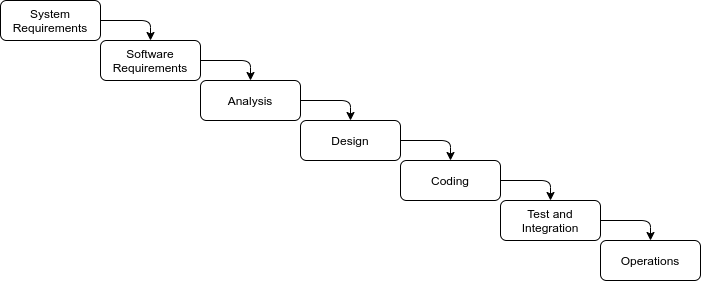
\includegraphics[width=1.0\textwidth]{images/WaterfallModel.png}
\end{figure}

\begin{figure}[h!]
    \caption{Agile Development Process Model}
    \label{image:agileModel}
    \centering
    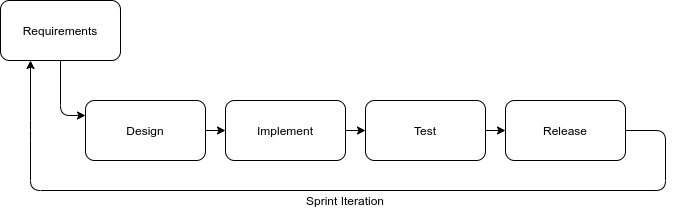
\includegraphics[width=1.0\textwidth]{images/AgileModel.png}
\end{figure}

\section{Project \& Time Management}
At an early stage in the project it was opted to use an issue tracking software to manage the workload, allocation of tasks, and to monitor the current stage of development.
\\ Initially Jira, by Atlassian, was examined, which was unfortunately a bit costly and had no education deals. Upon further digging YouTrack was found, which has the same ticket issuing capabilities as Jira, but was free for student use.
\subsection{YouTrack}
YouTrack is a browser-based, project management software, developed by JetBrains. It handles bug management and ticket issuing and tracking. This software was used in order to keep a handle on the current issue backlog and was monitored and managed by all members of the team. 

\begin{figure}[h!]
    \caption{Issue Matrix}
    \label{image:issuesMatrix}
    \centering
    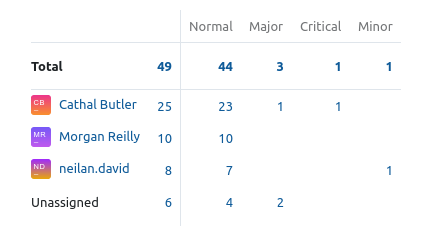
\includegraphics[width=1.0\textwidth]{images/IssuesMatrix.png}
\end{figure}

\begin{figure}[h!]
    \caption{Issues Per Assignee}
    \label{image:IPA}
    \centering
    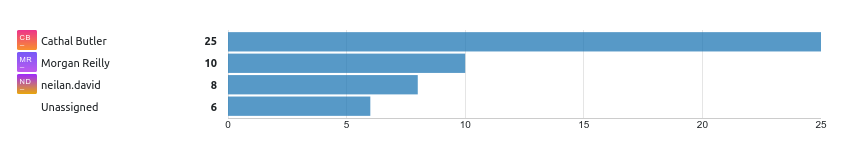
\includegraphics[width=1.0\textwidth]{images/IssuesPerAssignee.png}
\end{figure}

\begin{figure}[h!]
    \caption{Cumulative Flow Of Issues}
    \label{image:cumFlow}
    \centering
    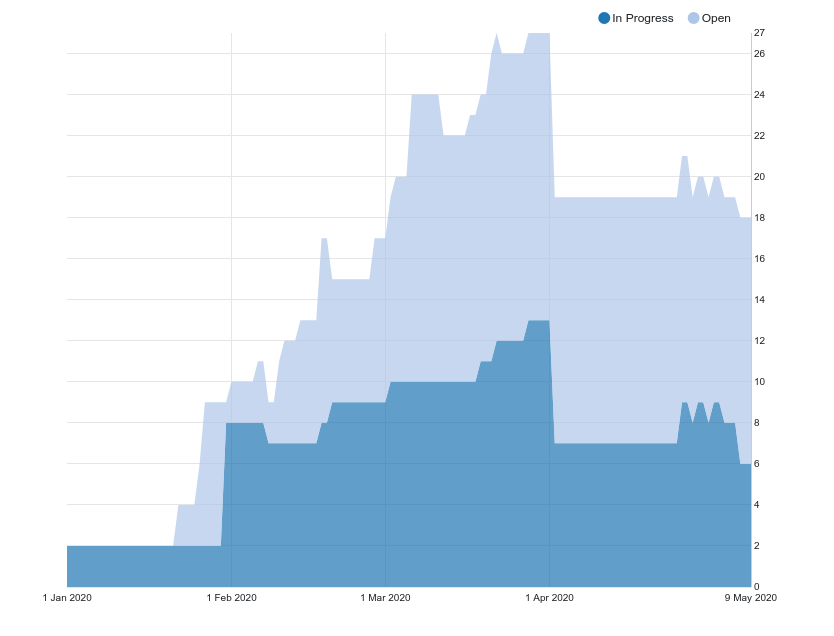
\includegraphics[width=1.0\textwidth]{images/FlowCumulative.png}
\end{figure}